%%%%%%%%%%%%%%%%%%%%%%%%%%%%%%%%%%%%%%%%%
% Journal Article
% LaTeX Template
% Version 1.3 (9/9/13)
%
% This template has been downloaded from:
% http://www.LaTeXTemplates.com
%
% Original author:
% Frits Wenneker (http://www.howtotex.com)
%
% License:
% CC BY-NC-SA 3.0 (http://creativecommons.org/licenses/by-nc-sa/3.0/)
%
%%%%%%%%%%%%%%%%%%%%%%%%%%%%%%%%%%%%%%%%%

%----------------------------------------------------------------------------------------
%	PACKAGES AND OTHER DOCUMENT CONFIGURATIONS
%----------------------------------------------------------------------------------------

\documentclass[twoside]{article}

\usepackage{lipsum} % Package to generate dummy text throughout this template
%\usepackage[showframe]{geometry}% http://ctan.org/pkg/geometry

\usepackage[sc]{mathpazo} % Use the Palatino font
\usepackage[T1]{fontenc} % Use 8-bit encoding that has 256 glyphs
\linespread{1.05} % Line spacing - Palatino needs more space between lines
\usepackage{microtype} % Slightly tweak font spacing for aesthetics
\usepackage{graphicx}
\usepackage[hmarginratio=1:1,top=32mm,columnsep=20pt]{geometry} % Document margins
\usepackage{multicol} % Used for the two-column layout of the document
\usepackage[hang, small,labelfont=bf,up,textfont=it,up]{caption} % Custom captions under/above floats in tables or figures
\usepackage{booktabs} % Horizontal rules in tables
\usepackage{float} % Required for tables and figures in the multi-column environment - they need to be placed in specific locations with the [H] (e.g. \begin{table}[H])
\usepackage{hyperref} % For hyperlinks in the PDF

\usepackage{lettrine} % The lettrine is the first enlarged letter at the beginning of the text
\usepackage{paralist} % Used for the compactitem environment which makes bullet points with less space between them

\usepackage{abstract} % Allows abstract customization
\renewcommand{\abstractnamefont}{\normalfont\bfseries} % Set the "Abstract" text to bold
\renewcommand{\abstracttextfont}{\normalfont\small\itshape} % Set the abstract itself to small italic text
%\usepackage{apacite}
\bibliographystyle{ieeetr}

\usepackage{titlesec} % Allows customization of titles
\renewcommand\thesection{\Roman{section}} % Roman numerals for the sections
\renewcommand\thesubsection{\Roman{subsection}} % Roman numerals for subsections
\titleformat{\section}[block]{\large\scshape\centering}{\thesection.}{1em}{} % Change the look of the section titles
\titleformat{\subsection}[block]{\large}{\thesubsection.}{1em}{} % Change the look of the section titles

\usepackage{fancyhdr} % Headers and footers
\pagestyle{fancy} % All pages have headers and footers
\fancyhead{} % Blank out the default header
\fancyfoot{} % Blank out the default footer
\fancyhead[C]{}
%Running title $\bullet$ November 2012 $\bullet$ Vol. XXI, No. 1} % Custom header text
\fancyfoot[RO,LE]{\thepage} % Custom footer text

%----------------------------------------------------------------------------------------
%	TITLE SECTION
%----------------------------------------------------------------------------------------

\title{\vspace{-15mm}\fontsize{24pt}{10pt}\selectfont\textbf{BioJS-HGV Viewer: A BioJS component for visualzing protein variants}} % Article title

\author{
\large
\textsc{Saket K Choudhary}\thanks{Molecular and Computational Biology, University of Southern California, Los Angeles, California, USA}\\[2mm] % Your name
\textsc{Leyla J Garcia, Andrew Nightingale}\thanks{European Bioinformatics Institute EMBL-EBI, Hinxton, Cambridge, CB10 1SD, UK}\\[2mm] % Your name
%\normalsize University of California \\ % Your institution
\normalsize \href{mailto:skchoudh@usc.edu}{skchoudh@usc.edu} % Your email address
\vspace{-5mm}
}
\date{}

%----------------------------------------------------------------------------------------

\begin{document}

\maketitle % Insert title

\thispagestyle{fancy} % All pages have headers and footers

%----------------------------------------------------------------------------------------
%	ABSTRACT
%----------------------------------------------------------------------------------------

\begin{abstract}

\noindent % \lipsum[1] % Dummy abstract text

Genomic studies have resulted in  catalogs of genetic variants in humans. Studying the pattern of damaging and non-damaging variants can not only help understand evolution but can also potentially improve human health by identifying the key driver elements.

We present BioJS-HGV Viewer, a BioJS component to represent and visualize genetic variants pooled from various sources. The component presents information at different levels allowing the end user to study the pattern of variations in detail in a user friendly manner. 

The code for BioJS-HGV Viewer is available at:\\ \url{https://github.com/saketkc/biojs-genetic-variation-viewer}.

A demo is available at: \url{http://saketkc.github.io/biojs}

\end{abstract}

%----------------------------------------------------------------------------------------
%	ARTICLE CONTENTS
%----------------------------------------------------------------------------------------

\begin{multicols}{2} % Two-column layout throughout the main article text

\section{Introduction}

\lettrine[nindent=0em,lines=3]{W} 
%orem ipsum dolor sit amet, consectetur adipiscing elit.
%\lipsum[2-3] % Dummy text
ith the advent of next-generation sequencing technologies, it has been possible to profile genomes in large numbers. One of the chief outcomes of such projects has been catalog of genetic variants such as dbSNP\cite{Smigielski2000} and COSMIC\cite{Forbes2011}. These catalogs contain publicly accessible sets of genetic variants found in humans which can be utilized to  study evolutionary relationships and disease specific variations. COSMIC database is a curated set of somatic mutations as observed in cancer samples. The number of such variations are   huge. dbSNP 129 had reportedly more than 14 million unique variants \cite{ncbiweb}. The availability of data at such a large scale makes the analysis challenging.

Any exploratory attempt at making sense of the variation data would involve visualizing the variants across the genome to determine specific sites, if any where the mutations are more frequent or are absent completely. 
 BioJS-HGV Viewer is a BioJS \cite{Corpas2014} component developed to visualize genetic variants in a comprehensive manner.BioJS is an open source project providing various components to visualize biological data. These components use javascript for rendering visualization. The visualizations are web based and hence are absolutely platform independent.
 
 
%------------------------------------------------

\section{Methods}
The functionality provided by BioJS-HGV Viewer has two parts:\\
\begin{compactitem}
\item Overview
\item Detailed or Zoomed View
\end{compactitem}

%\begin{figure*}
%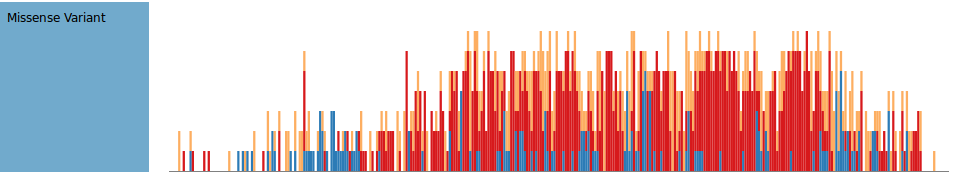
\includegraphics[width=\linewidth]{openview0}
%\caption{'Overview' of genetic variants as shown in by HGV viewer}
%\end{figure*}

%\begin{figure*}
%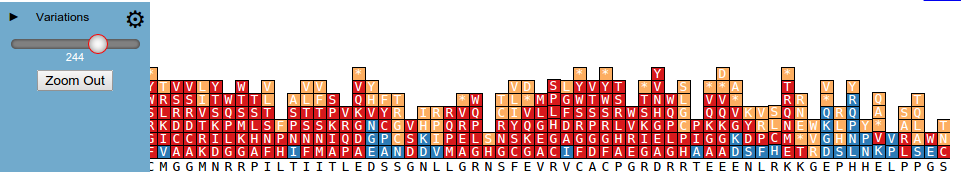
\includegraphics[width=\linewidth]{zoomed0}
%\caption{'Detailed view' of genetic variants. The SIFT/Polyphen scores and associated %information with the mutations is rendered using tooltips(not shown here)}
%\end{figure*}
\begin{figure*}
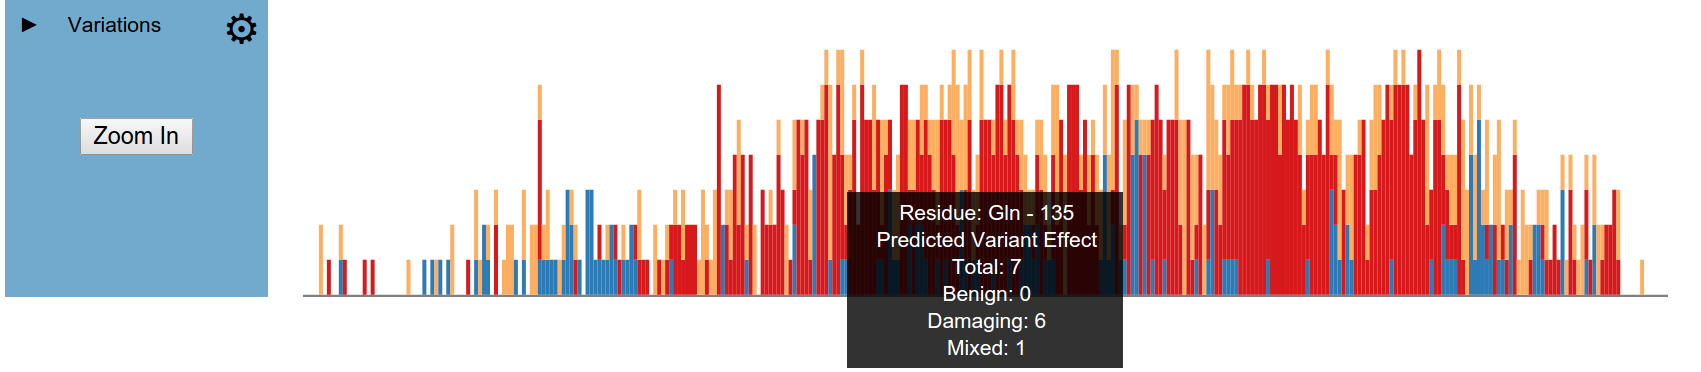
\includegraphics[width=\linewidth]{overview_withtooltip}
\caption{'Overview' of genetic variants as shown in by HGV viewer. Tooltips are used to display the number of mutations in benign, damaging and mixed categories.}
\end{figure*}
\begin{figure*}
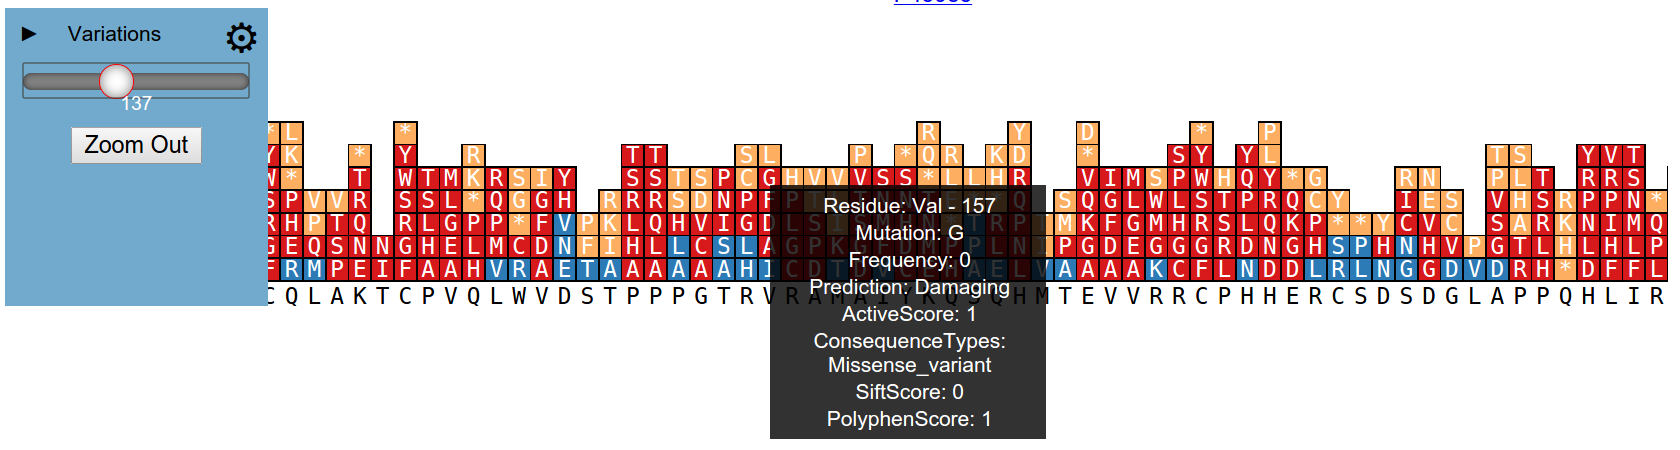
\includegraphics[width=\linewidth]{zoomed_withtooltip}
\caption{'Detailed view' of genetic variants. The SIFT/Polyphen scores and associated information with the mutations is rendered using tooltips}
\end{figure*}



%------------------------------------------------

\section{Results}

%\begin{table}[H]
%\caption{Example table}
%\centering
%\begin{tabular}{llr}
%\toprule
%\multicolumn{2}{c}{Name} \\
%\cmidrule(r){1-2}
%First name & Last Name & Grade \\
%\midrule
%John & Doe & $7.5$ \\
%Richard & Miles & $2$ \\
%\bottomrule
%\end{tabular}
%\end{table}


%------------------------------------------------

\section{Discussion}

\subsection{Subsection One}



\subsection{Subsection Two}



%----------------------------------------------------------------------------------------
%	REFERENCE LIST
%----------------------------------------------------------------------------------------



\bibliography{biojs_paper}


%----------------------------------------------------------------------------------------

\end{multicols}

\end{document}